\section{Basics of mega-modeling}\label{sec:BasicsOfMegamodeling}
The second topic of current research on which we need basic knowledge to understand the coming sections is mega-modeling. The term mega-model is somewhat ambiguous as it commonly refers to models using other models as their elements. But the term model is not used in a restrictive manner \cite{MEGAL2}, it may be interpreted as intuitive models, elements of such models, meta-models describing such models and moreover the term may be used for mega-models itself as depicted in Figure \ref{fig:BoradSenseMegaModel}, so mega-models could actually describe mega-mega-models or even mega*-models. And to make things a little bit more confusing mega-models may also be defined by meta-models.

\begin{figure}
\centering
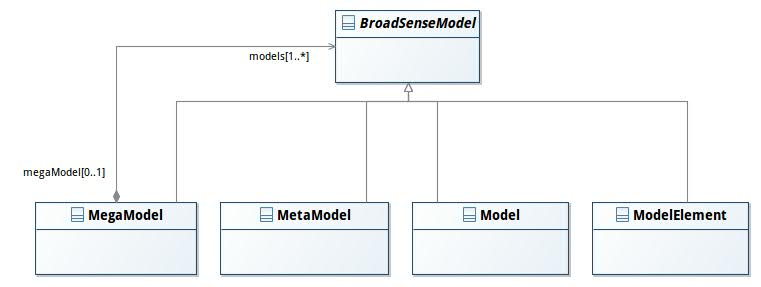
\includegraphics[width=\textwidth]{BroadSenseMegaModel.jpg}
\caption{Mega-models in a broad sense}
\label{fig:BoradSenseMegaModel}
\end{figure}

\subsection{Mega-model usage}\label{subsec:MegaModelUsage}
Unsurprisingly mega-models are meant to be used for large-scale modeling, i.e. models of big enterprise systems \cite{TowardsAMegamodel}. Such systems are ecosystem-like environments consisting of various different technologies interacting with each other. Especially regarding this aspect of systems one can make use of mega-models to investigate the dependencies of involved \textit{technological spaces} \cite{MEGAL1}\cite{MEGAL2}\cite{TowardsAMegamodel}. However the use of mega-models may not only be indicated by system size. Even minimal static \footnote{static in a sense that content data is not provided dynamically, i.e. form of databases} web-pages can use a multitude of technologies in form of
\begin{itemize}
\item software languages like HTML, CSS and JavaScript (nowadays CSS also may conform to corresponding LESS or SASS code),
\item software APIs likes JQuery, Angular.js, etc.,
\item infrastructure components like server and client/browser, 
\item and protocols like HTTP(S) or FTP.
\end{itemize}
Enhancing the web-page with server side logic might add the technological spaces of PHP-ware, Java-ware and/or SQL-ware.

Another use case or need for mega-models arises implicitly when one wants to build MDE supporting tools. MDE-tools provide functionalities to create and maintain digital representations of models, meta-models and model- transformations. To do so, such tools need to implement a meta-model capable of these three (ore more) aspects, whose object instances would in fact be some sort of mega-models. Seibel et al. \cite{DHMM} created a prototype which is able of managing traceability links between models and model-elements by utilizing a meta-mega-model.

\subsection{The MDE-Mega-Model}\label{subsec:TheMDEMegaModel}
One particular mega-model we want to point out is the MDE-Mega-Model (Figure \ref{fig:TheMDEMegaModel}) by Favre et al. \cite{TowardsAMegamodel}.This approach aims to model MDE evolution processes. Although it is not yet complete, it already proves to be a powerful help analyzing technological spaces. 

\begin{figure}
\centering
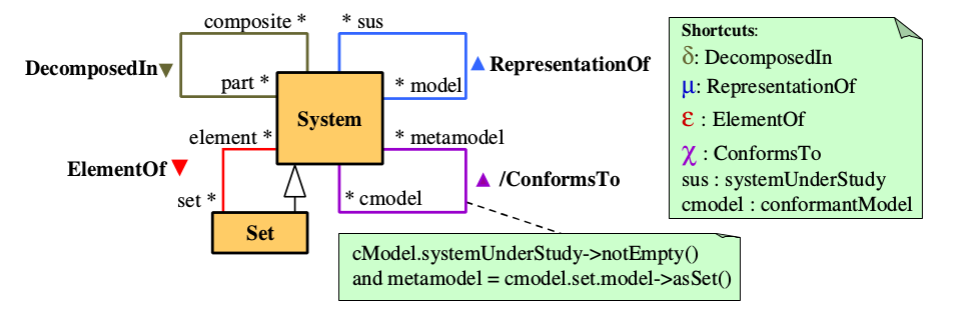
\includegraphics[width=\textwidth]{MDE-MegaModel.png}
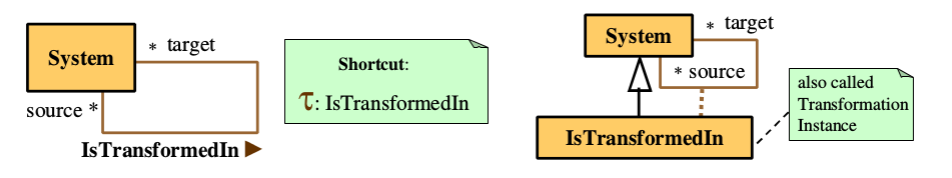
\includegraphics[width=\textwidth]{MDE-MegaModel-Transformations.png}
\caption{The MDE-Mega-Model by Favre et al. \cite{TowardsAMegamodel}}
\label{fig:TheMDEMegaModel}
\end{figure}

The other reason to introduce this mega-model here is due to its concise nature and high level of abstraction regarding MDE. This makes it an ideal framework for analyzing other concrete mega-models.

Favre et al. identify five relations concerning systems which we will now explain in short:

\subsubsection{systems} At first we need to clarify the term \textit{system}. Favre et al. state: \textit{''A system is the primary element of discourse when talking about MDE''}, although the terms usage may not be important as everything can be seen as some kind of system \cite{TowardsAMegamodel}. This is exemplified with the trigonometric system $\pi$ (meaning the real number). For the sake of simplicity and not repeating examples we may just think of a system as the \textit{thing of interest}.

\subsubsection{$\delta$ (\texttt{DecomposedIn})}
Decomposition is a structural relationship which denotes that a \textit{composite} can be \texttt{DecomposedIn} a \textit{part}, or in set-theoretic notation: 
\begin{center}
\textit{composite} $\delta$ \textit{part} or $(composite, part) \in \delta$
\end{center}
Example: A directory in a file system tree contains simple files and other directories, so its safe to say: \texttt{dir} $\delta$ \texttt{file} and \texttt{dir} $\delta$ \texttt{dir}. The latter also illustrates the recursive notion of this relation.

\subsubsection{$\mu$ (\texttt{RepresentationOf})}
Representation is a descriptive relationship denoting a \textit{model} as a \texttt{RepresentationOf} of a \textit{system under study}. We write:
\begin{center}
\textit{model} $\mu$ \textit{sus}
or 
(\textit{model},\textit{sus}) $\in\mu$
\end{center}
Again, we do not care that much about the term \textit{system}, for \textit{model} on the other hand we think of it as abstraction and/or simplification of such systems.
Example: As directories contain $n$ files, a list of files can be the representation of a directory: \texttt{[file0,file1,...]} $\mu$ \texttt{dir}.

\subsubsection{$\varepsilon$ (\texttt{ElementOf})}
This is simply the set-theoretic $\in$ relationship, so an \textit{element} is \texttt{ElementOf} a \textit{set}. In greek notation:
\begin{center}
\textit{element} $\varepsilon$ \textit{set}
or 
(\textit{element},\textit{set}) $\in\varepsilon$
\end{center}
Example: \texttt{FOO := (/foo)+}  may be the set of all Unix-files following the this pattern ( \texttt{FOO = \{ /foo, /foo/foo, /foo/foo/foo, ... \} } ), so \texttt{/foo} $\varepsilon$ \texttt{FOO}.

\subsubsection{$\chi$ (\texttt{ConformsTo})} Conformance adds the notion of meta-models, where a \textit{conformantModel} \texttt{ConformsTo} a \textit{metamodel}.
\begin{center}
\textit{cmodel} $\chi$ \textit{metamodel}
or 
(\textit{cmodel},\textit{metamodel}) $\in\chi$
\end{center}
Example: \texttt{(/foo)+} is a model for \texttt{FOO}, \texttt{/foo(/foo)*} is also one, so we have \texttt{(/foo)+} $\mu$ \texttt{FOO}. Both are regular expression describing the same set of strings and thus have to obey the syntax rules for regular expressions (\texttt{RegExp}), or in the notation of this mega-model: \texttt{(/foo)+} $\chi$ \texttt{RegExp}.

\subsubsection{$\tau$ (\texttt{IsTransformedIn})}
Transformations play a very important role in MDE because the benefit of just being able to statically describe systems is limited. Additionally we need the ability to model the progress of a development process. But this is relatively simple to achieve by applying the well known concept of functions to this mega-model. So we may say a \textit{source} \texttt{IsTransformedIn} a \textit{target}, we think \textit{source} $\mapsto$ \textit{target} and write:
\begin{center} 
\textit{source} $\tau$ \textit{target}
or 
(\textit{source},\textit{target}) $\in\tau$
\end{center}
Example: One transformation class of particular interest are model transformations. Given the established model \texttt{(/foo)+}, we might have it transformed to the model \texttt{(/bar)+}. This is denoted as  \texttt{(/foo)+} $\tau$ \texttt{(/bar)+} or (\texttt{(/foo)+}, \texttt{(/bar)+}). The latter is also called \textit{transformation instance/application}.
\newline

The MDE-Mega-Model and the important role of transformations and \textit{transformation systems} can be explored in more detail in the paper by Favre et al. \cite{TowardsAMegamodel}. It also offers some insights on the correlation of (formal) languages and models, which enables a higher point of view on software in general. However, for this paper and its discussion of traceability the short introduction above is sufficient.

